\documentclass[aspectratio=169, table]{beamer}

\usepackage{array}
\usepackage{colortbl}
\usepackage{tabularx}
\usepackage{xcolor}
\usepackage{tikz}
\usetikzlibrary{arrows.meta, positioning, calc, fit}

\makeatletter
\def\input@path{{../theme/}}
\makeatother
\graphicspath{{../theme/}{../../figures/}}
\usetheme{Pradita}

\newcommand{\sectionframe}[1]{%
  \begin{frame}{\hfill}
    \centering
    \Huge{\textbf{#1}}
  \end{frame}
}

\newcommand{\takeaway}[1]{%
  \vspace{4pt}
  {\footnotesize #1}
}

\title{\huge Lapisan Bisnis\\
  \vspace{8pt}
  pada ArchiMate}
\subtitle{IT30713 - Enterprise \& Platform Architecture}
\author{\textbf{Alfa Yohannis}}
\date{20 Juni 2026}

\begin{document}

\frame{\titlepage}

\begin{frame}[fragile]
  \frametitle{Contents}
  \vspace{20pt}
  \begin{columns}[t]
    \column{0.5\textwidth}
    \tableofcontents[sections={1-4}]

    \column{0.5\textwidth}
    \tableofcontents[sections={5-8}]
  \end{columns}
\end{frame}

\begin{frame}{\hfill}
  \centering
  \Huge{\textbf{Strategi sudah dipilih---bagaimana bisnis mewujudkannya?}}
\end{frame}

% ============================================================
\section{Orientasi Bab}
\sectionframe{Orientasi Bab}

\begin{frame}{Tujuan Pembelajaran}
  \vspace{6pt}
  \begin{itemize}
    \item Menjelaskan elemen \textbf{lapisan bisnis} ArchiMate: layanan, proses,
          peran/aktor, fungsi, dan objek bisnis.
    \item Menyusun \textbf{capability map} yang membedakan kapabilitas inti,
          pendukung, dan tata kelola.
    \item Memetakan \textbf{value stream} dan \textbf{proses bisnis} transfer
          untuk menemukan titik masalah dan kebutuhan data.
    \item Menempatkan analisis dalam \textbf{TOGAF ADM Fase B}: arsitektur bisnis
          \emph{baseline}, \emph{target}, dan analisis kesenjangan.
  \end{itemize}
  \takeaway{Arah sesi: dari ``strategi apa'' menuju ``bagaimana bisnis
  menjalankannya'' secara konkret dan dapat dianalisis.}
\end{frame}

\begin{frame}{Ringkasan Awal Bab}
  \vspace{6pt}
  \begin{itemize}
    \item Lapisan strategi memberi arah; \textbf{lapisan bisnis} memberi
          struktur perilaku yang mewujudkannya.
    \item Tiga artefak inti: \textbf{capability map}, \textbf{value stream \&
          proses}, dan \textbf{model layanan} bisnis.
    \item Studi kasus berjalan: rel \textbf{API Transfer Dana} Bank Wanua---dari
          inisiasi instruksi sampai rekonsiliasi.
    \item Keluaran bab memperkuat \textbf{analisis} dan \textbf{Literature Review
          v1} makalah.
  \end{itemize}
  \takeaway{Lapisan bisnis menurunkan strategi menjadi layanan, proses, dan peran
  yang dapat ditelusuri.}
\end{frame}


% ============================================================
\section{Mengapa Lapisan Bisnis}
\sectionframe{Mengapa Lapisan Bisnis}

\begin{frame}{Posisi Lapisan Bisnis dalam ArchiMate}
  \vspace{2pt}
  \centering
  \scalebox{0.74}{
    \begin{tikzpicture}[
      font=\small\bfseries,
      node distance=2.2mm,
      layer/.style={draw, rounded corners=1.5mm, align=left, minimum width=82mm,
        minimum height=10mm, inner xsep=4mm},
      strat/.style={layer, fill=orange!16},
      biz/.style={layer, fill=praditagreen!30, draw=praditagreen, line width=0.5mm},
      app/.style={layer, fill=blue!14},
      tech/.style={layer, fill=gray!18},
      impl/.style={layer, fill=orange!10},
    ]
      \node[strat] (s) {STRATEGI\\
        \footnotesize\mdseries Sumber daya, kapabilitas, arah tindakan, value stream};
      \node[biz, below=of s] (b) {BISNIS \quad$\leftarrow$ \emph{fokus sesi ini}\\
        \footnotesize\mdseries Aktor, peran, proses, fungsi, layanan, objek bisnis};
      \node[app, below=of b] (a) {APLIKASI\\
        \footnotesize\mdseries Komponen, layanan, dan antarmuka aplikasi};
      \node[tech, below=of a] (t) {TEKNOLOGI (\& FISIK)\\
        \footnotesize\mdseries Node, perangkat, jaringan, \emph{system software}};
      \node[impl, below=of t] (i) {IMPLEMENTASI \& MIGRASI\\
        \footnotesize\mdseries \emph{Work package}, \emph{deliverable},
        \emph{plateau}, \emph{gap}};
      \node[draw, rounded corners=2mm, fill=purple!22, align=center,
        text width=16mm, minimum height=60mm, right=5mm of a, font=\bfseries]
        (mot) {M\\O\\T\\I\\V\\A\\S\\I\\[2mm]\footnotesize\mdseries (mengapa)};
    \end{tikzpicture}
  }

  \takeaway{Lapisan bisnis \emph{menerjemahkan} visi dan strategi menjadi
  perilaku; dipetakan ke fase \textbf{B (Arsitektur Bisnis)} TOGAF ADM.}
\end{frame}



\begin{frame}{Antara Strategi dan Rancangan Teknis}
  \vspace{6pt}
  \begin{itemize}
    \item Tanpa lapisan bisnis, makalah melompat dari visi langsung ke aplikasi
          dan basis data.
    \item Lapisan bisnis menjawab: \emph{layanan} apa yang ditawarkan,
          \emph{proses} apa yang menjalankannya, \emph{siapa} aktornya, dan
          \emph{data} apa yang diolah.
    \item Di sinilah \textbf{kapabilitas} strategi menjadi konkret dan titik
          masalah (\emph{pain point}) menjadi terlihat.
  \end{itemize}
  \takeaway{Bagi pembaca non-TI: lapisan bisnis adalah ``cara kerja''
  organisasi---sebelum bicara sistem.}
\end{frame}

% ============================================================
\section{TOGAF ADM Fase B}
\sectionframe{TOGAF ADM Fase B:\\ Arsitektur Bisnis}

\begin{frame}{Siklus TOGAF ADM}
  \vspace{8pt}
  \begin{columns}[c]
    \column{0.4\textwidth}
    \centering
    \scalebox{0.85}{
      \begin{tikzpicture}[
        font=\footnotesize\bfseries,
        phase/.style={circle, draw=praditagreen, line width=0.4mm,
          fill=praditagreen!15, minimum size=11mm, inner sep=0pt},
        reqman/.style={circle, draw=blueColor, line width=0.4mm, fill=blueColor!15,
          minimum size=21mm, inner sep=1pt, align=center, font=\scriptsize\bfseries},
        prelim/.style={circle, draw=orange!80!black, line width=0.4mm,
          fill=orange!25, minimum size=13mm, inner sep=0pt, align=center,
          font=\scriptsize\bfseries},
        ring/.style={-Latex, draw=praditagreen!75, line width=0.4mm},
        spoke/.style={draw=blueColor!35, line width=0.25mm},
      ]
        \node[reqman] (rm) at (0,0) {Manajemen\\Requirements};
        \foreach \ang/\lab in {90/A, 45/B, 0/C, -45/D, -90/E, -135/F, 180/G, 135/H}
          \node[phase] (\lab) at (\ang:2.6cm) {\lab};
        \node[prelim] (P) at (90:4.1cm) {Prelim.};
        \foreach \lab in {A,B,C,D,E,F,G,H} \draw[spoke] (\lab) -- (rm);
        \foreach \a/\b in {A/B, B/C, C/D, D/E, E/F, F/G, G/H, H/A}
          \draw[ring] (\a) to[bend left=12] (\b);
        \draw[ring, draw=orange!80!black] (P) -- (A);
        \node[phase, fill=orange!45, line width=0.7mm] at (45:2.6cm) {B};
      \end{tikzpicture}
    }
    \column{0.6\textwidth}
    {\footnotesize TOGAF (\emph{The Open Group Architecture Framework}); ADM
    (\emph{Architecture Development Method})---metode pengembangan arsitektur
    dengan siklus berulang.\par}
    \vspace{5pt}
    \footnotesize
    \begin{itemize}\setlength{\itemsep}{1.0pt}
      \item \textbf{Prelim.}---Persiapan \& prinsip
      \item \textbf{A}---Visi Arsitektur
      \item \textbf{\textcolor{orange!80!black}{B---Arsitektur Bisnis}}
            $\leftarrow$ \emph{fokus sesi ini}
      \item \textbf{C}---Arsitektur Sistem Informasi (Data \& Aplikasi)
      \item \textbf{D}---Arsitektur Teknologi
      \item \textbf{E}---Peluang \& Solusi
      \item \textbf{F}---Perencanaan Migrasi
      \item \textbf{G}---Tata Kelola Implementasi
      \item \textbf{H}---Manajemen Perubahan Arsitektur
      \item \textbf{Manajemen Requirements}---di pusat, menyetir semua fase
    \end{itemize}
  \end{columns}
\end{frame}

\begin{frame}{Fase B: Lima Langkah}
  \vspace{2pt}
  \footnotesize
  \begin{columns}[t]
    \column{0.5\textwidth}
    \textbf{Apa \& Mengapa}
    \begin{itemize}\setlength{\itemsep}{2.5pt}
      \item Fase A menetapkan \emph{visi}; Fase B menerjemahkannya menjadi
            arsitektur bisnis konkret.
      \item Menghasilkan dua potret: \emph{baseline} (kini) dan \emph{target}
            (dituju).
      \item Selisihnya = \textbf{analisis kesenjangan} $\rightarrow$ bahan peta
            jalan.
    \end{itemize}
    \column{0.5\textwidth}
    \textbf{Lima Langkah}
    \begin{enumerate}\setlength{\itemsep}{2.5pt}
      \item Ruang lingkup \& prinsip bisnis.
      \item Arsitektur bisnis \textbf{baseline}.
      \item Arsitektur bisnis \textbf{target}.
      \item Analisis \textbf{kesenjangan}.
      \item Masukan ke Fase C (sistem informasi).
    \end{enumerate}
  \end{columns}
  \vspace{2pt}
  \takeaway{Keluaran Fase B: capability map, model layanan \& proses, dan
  analisis kesenjangan---jembatan dari visi ke rancangan sistem.}
\end{frame}

% ============================================================
\section{Elemen Lapisan Bisnis}
\sectionframe{Elemen Lapisan Bisnis}

\begin{frame}{Jenis Elemen dan Simbolnya di Archi}
  \vspace{6pt}
  \begin{columns}[c]
    \column{0.56\textwidth}
    \centering
    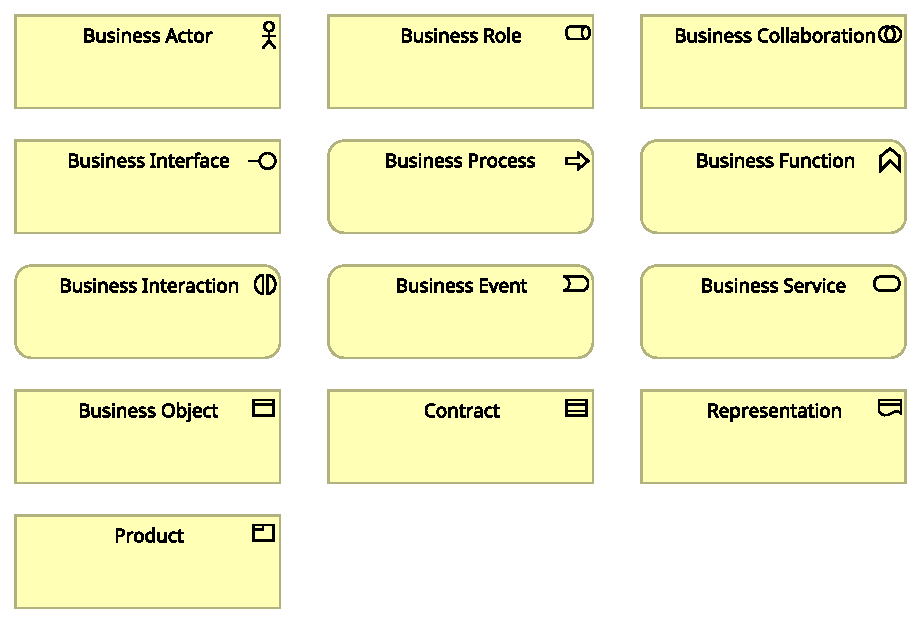
\includegraphics[width=\linewidth]{business-legend.pdf}
    \column{0.44\textwidth}
    \footnotesize
    \begin{itemize}\setlength{\itemsep}{2.5pt}
      \item \textbf{Aktor / Peran} -- siapa yang menjalankan.
      \item \textbf{Antarmuka} -- titik akses (API, kanal).
      \item \textbf{Proses / Fungsi} -- perilaku yang dijalankan.
      \item \textbf{Layanan} -- yang ditawarkan ke pengguna.
      \item \textbf{Objek bisnis} -- informasi yang diolah.
      \item \textbf{Produk / Kontrak} -- bungkusan \& perjanjian.
    \end{itemize}
  \end{columns}
  \takeaway{Elemen bisnis memakai persegi panjang kuning muda; ikon pojok
  membedakan jenisnya.}
\end{frame}

\begin{frame}{Membedakan Elemen Bisnis}
  \vspace{6pt}
  \begin{itemize}
    \item \textbf{Layanan (service):} apa yang ditawarkan---``Layanan Transfer
          Dana''.
    \item \textbf{Proses (process):} urutan kegiatan yang menghasilkan layanan.
    \item \textbf{Fungsi (function):} pengelompokan perilaku menurut kemampuan.
    \item \textbf{Peran/aktor:} siapa yang menjalankan.
    \item \textbf{Objek bisnis:} informasi---``Instruksi Transfer'', ``Hasil
          Penyaringan''.
  \end{itemize}
  \takeaway{Satu kapabilitas dapat muncul di banyak proses; satu proses dapat
  memerlukan banyak kapabilitas.}
\end{frame}

\begin{frame}{}
  \centering
  \vspace{1mm}
  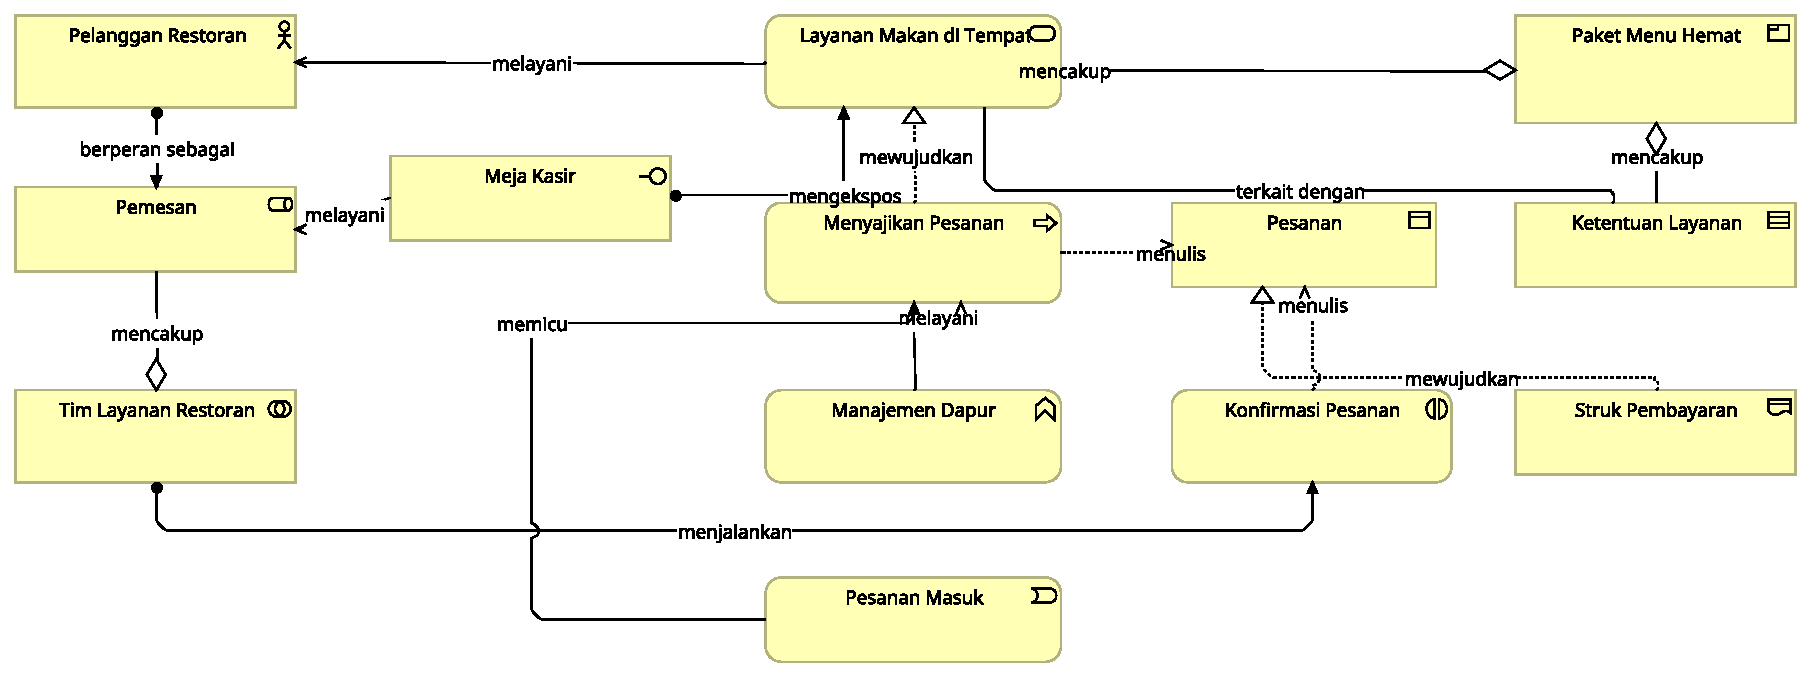
\includegraphics[width=\textwidth,height=.82\textheight,keepaspectratio]{business-contoh.pdf}\\
  {\scriptsize Contoh interaksi ke-13 jenis elemen bisnis (kasus restoran cepat saji).}
\end{frame}

% ============================================================
\section{Capability Map}
\sectionframe{Business Capability \& Capability Map}

\begin{frame}{Capability Map Rel Transfer Bank Wanua}
  \vspace{6pt}
  \centering
  \scalebox{0.82}{
    \begin{tikzpicture}[
      capnode/.style={rectangle, rounded corners=1.5mm, draw=praditagreen,
        fill=praditagreen!10, thick, align=center, text width=30mm, minimum height=10mm},
      core/.style={rectangle, rounded corners=1.5mm, draw=orange!80!black,
        fill=orange!18, thick, align=center, text width=30mm, minimum height=10mm},
      support/.style={rectangle, rounded corners=1.5mm, draw=blue!70!black,
        fill=blue!10, thick, align=center, text width=30mm, minimum height=10mm},
      layer/.style={font=\small\bfseries, align=right, text width=22mm, anchor=east}
    ]
      \node[layer] at (-0.6,2.6) {Strategis\\\& tata kelola};
      \node[capnode] (s1) at (1.4,2.6) {Tata kelola API};
      \node[capnode] (s2) at (4.8,2.6) {Manajemen risiko\\\& kepatuhan};
      \node[capnode] (s3) at (8.2,2.6) {Tata kelola data};
      \node[layer] at (-0.6,1.0) {Kapabilitas\\inti};
      \node[core] (c1) at (1.4,1.0) {Inisiasi \&\\otorisasi transfer};
      \node[core] (c2) at (4.8,1.0) {Penyaringan AML\\\& limit};
      \node[core] (c3) at (8.2,1.0) {Penyelesaian \&\\kliring (BI-FAST)};
      \node[layer] at (-0.6,-0.6) {Kapabilitas\\pendukung};
      \node[support] (p1) at (1.4,-0.6) {Notifikasi};
      \node[support] (p2) at (4.8,-0.6) {Rekonsiliasi};
      \node[support] (p3) at (8.2,-0.6) {Manajemen\\mitra \& kanal};
      \draw[gray!45, rounded corners=2mm] (-3.0,-1.3) rectangle (10.1,3.25);
    \end{tikzpicture}
  }

  \takeaway{Kapabilitas $\neq$ proses: kapabilitas = \emph{kemampuan yang harus
  ada}; proses = \emph{urutan aktivitas}. Peta ini menyetir prioritas.}
\end{frame}

% ============================================================
\section{Value Stream \& Proses}
\sectionframe{Value Stream \& Proses Bisnis}

\begin{frame}{Value Stream \& Proses Transfer Dana}
  \vspace{4pt}
  \centering
  \scalebox{0.72}{
    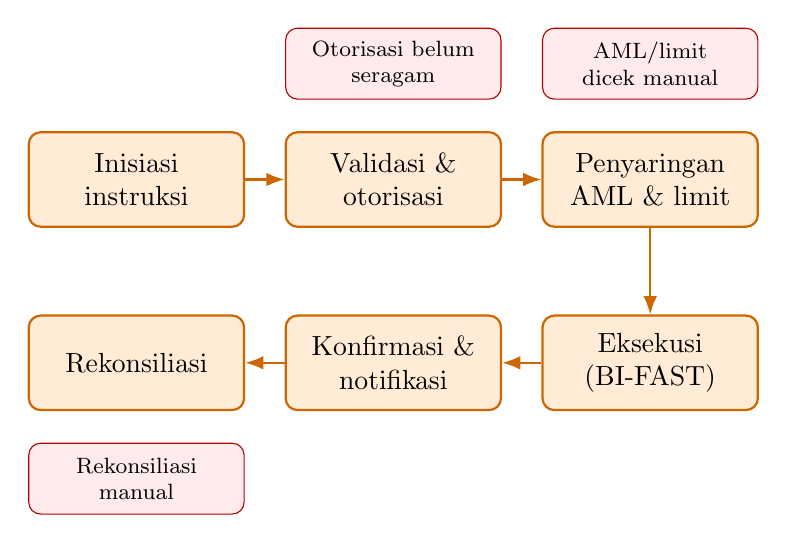
\begin{tikzpicture}[
      stage/.style={rectangle, rounded corners=1.5mm, draw=orange!80!black,
        fill=orange!16, thick, align=center, text width=25mm, minimum height=12mm},
      pain/.style={rectangle, rounded corners=1.5mm, draw=red!70!black,
        fill=red!8, align=center, text width=25mm, minimum height=9mm, font=\footnotesize},
      link/.style={-Latex, thick, draw=orange!80!black}
    ]
      \node[stage] (s1) {Inisiasi\\instruksi};
      \node[stage, right=5mm of s1] (s2) {Validasi \&\\otorisasi};
      \node[stage, right=5mm of s2] (s3) {Penyaringan\\AML \& limit};
      \node[stage, below=11mm of s3] (s4) {Eksekusi\\(BI-FAST)};
      \node[stage, left=5mm of s4] (s5) {Konfirmasi \&\\notifikasi};
      \node[stage, left=5mm of s5] (s6) {Rekonsiliasi};
      \draw[link] (s1) -- (s2);
      \draw[link] (s2) -- (s3);
      \draw[link] (s3) -- (s4);
      \draw[link] (s4) -- (s5);
      \draw[link] (s5) -- (s6);
      \node[pain, above=4mm of s2] {Otorisasi belum\\seragam};
      \node[pain, above=4mm of s3] {AML/limit\\dicek manual};
      \node[pain, below=4mm of s6] {Rekonsiliasi\\manual};
    \end{tikzpicture}
  }

  \takeaway{\emph{Pain point} menautkan kapabilitas dengan masalah nyata: titik
  inilah yang menjadi fokus perbaikan dan kebutuhan sistem.}
\end{frame}



\begin{frame}{Baseline $\rightarrow$ Target (Bank Wanua)}
  \vspace{2pt}
  \scriptsize
  \setlength{\extrarowheight}{2pt}
  \arrayrulecolor{black!65}\setlength{\arrayrulewidth}{0.4pt}
  \begin{tabularx}{\textwidth}{|p{0.26\textwidth}|X|}
    \hline
    \rowcolor{praditagreen!18}
    \textbf{Langkah Fase B} & \textbf{Artefak pada kasus Bank Wanua} \\
    \hline
    Ruang lingkup \& prinsip & Rel API Transfer Dana; patuh SNAP BI, API sebagai produk, keamanan sejak awal. \\
    \hline
    Baseline & Transfer sebagian batch/manual; otorisasi belum seragam; AML \& rekonsiliasi manual. \\
    \hline
    Target & Layanan transfer real-time; proses terstandardisasi; penyaringan \& rekonsiliasi otomatis. \\
    \hline
    Analisis kesenjangan & Kapabilitas \emph{dibangun} vs.\ \emph{diperbaiki} (lihat capability map). \\
    \hline
    Masukan Fase C & Layanan AML, mesin rekonsiliasi, integrasi BI-FAST. \\
    \hline
  \end{tabularx}
  \vspace{4pt}
  \takeaway{Kesenjangan baseline--target adalah inti argumen perubahan dalam
  makalah.}
\end{frame}

\begin{frame}{}
  \centering
  \vspace{1mm}
  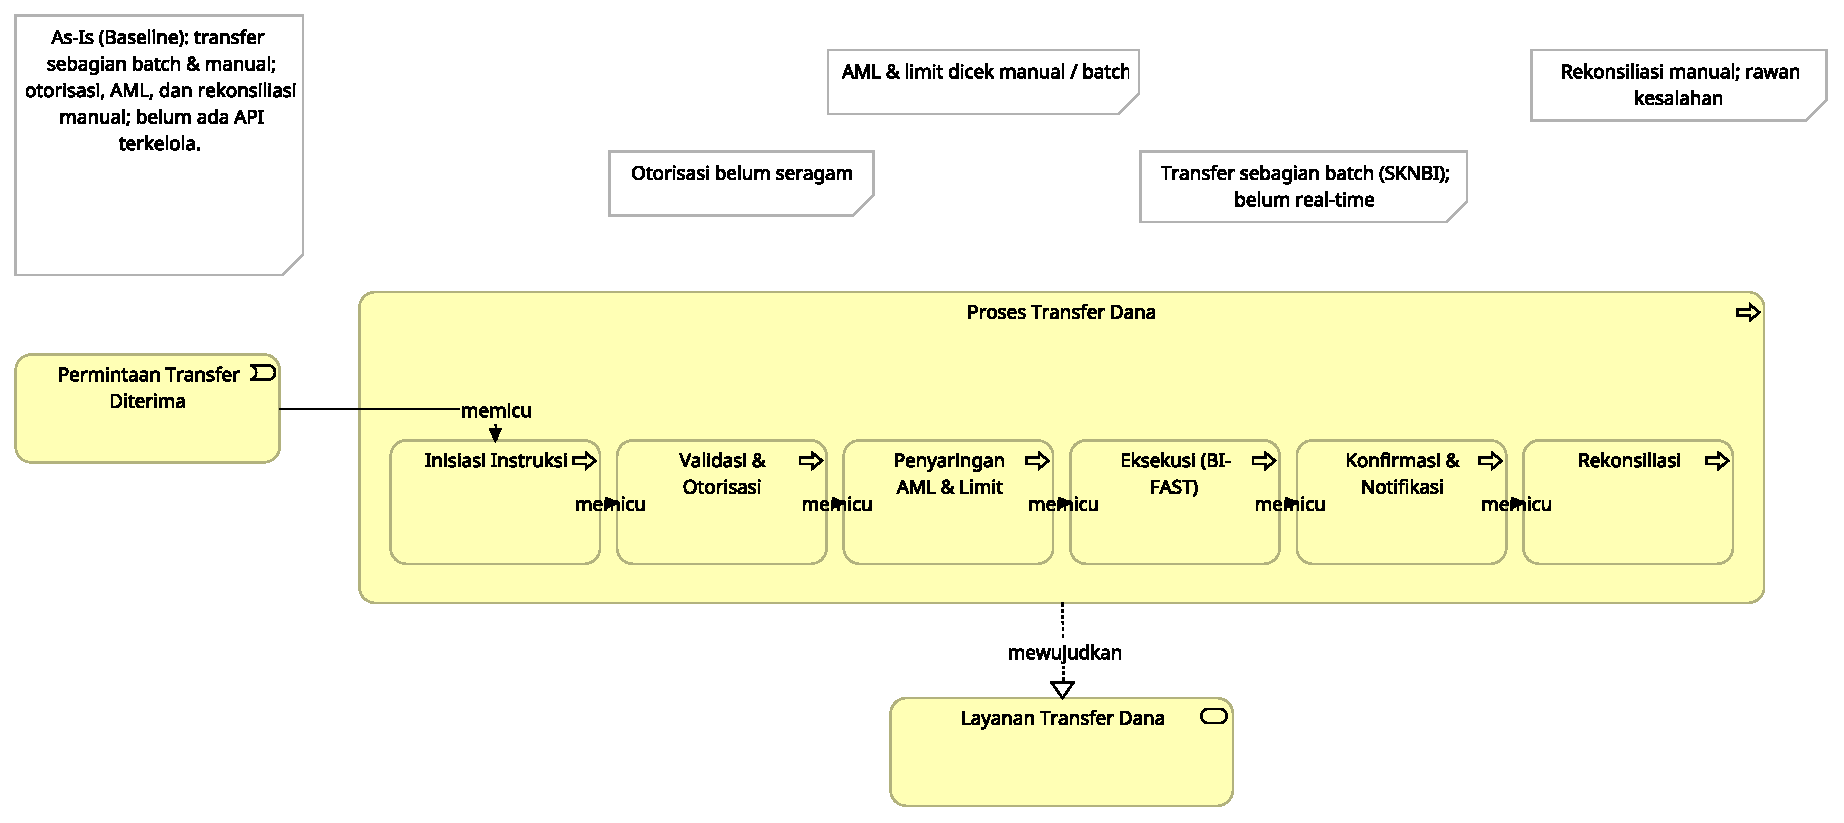
\includegraphics[width=\textwidth,height=.82\textheight,keepaspectratio]{business-asis.pdf}\\
  {\scriptsize \textbf{As-Is (Baseline):} transfer sebagian batch \& manual;
  otorisasi, AML, dan rekonsiliasi manual.}
\end{frame}

\begin{frame}{}
  \centering
  \vspace{1mm}
  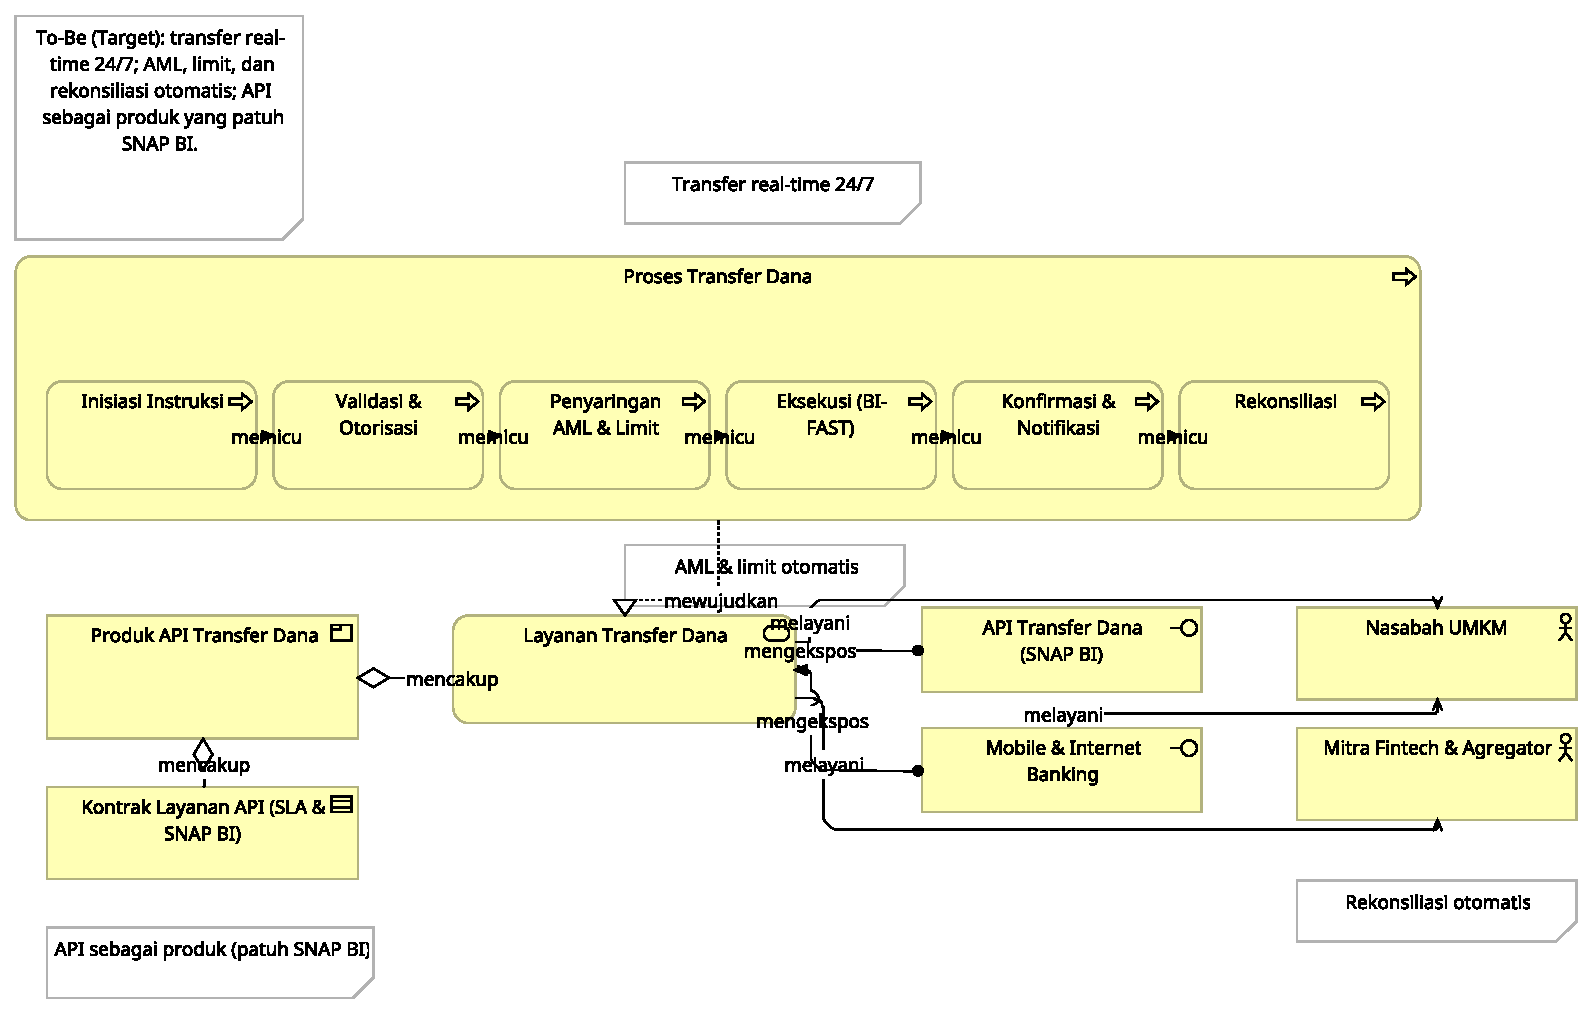
\includegraphics[width=\textwidth,height=.82\textheight,keepaspectratio]{business-tobe.pdf}\\
  {\scriptsize \textbf{To-Be (Target):} transfer real-time 24/7; AML, limit, dan
  rekonsiliasi otomatis; API sebagai produk patuh SNAP BI.}
\end{frame}

% ============================================================
\section{Studi Kasus: Model Bisnis di Archi}
\sectionframe{Studi Kasus:\\ Model Bisnis Transfer di Archi}

\begin{frame}{}
  \centering
  \vspace{1mm}
  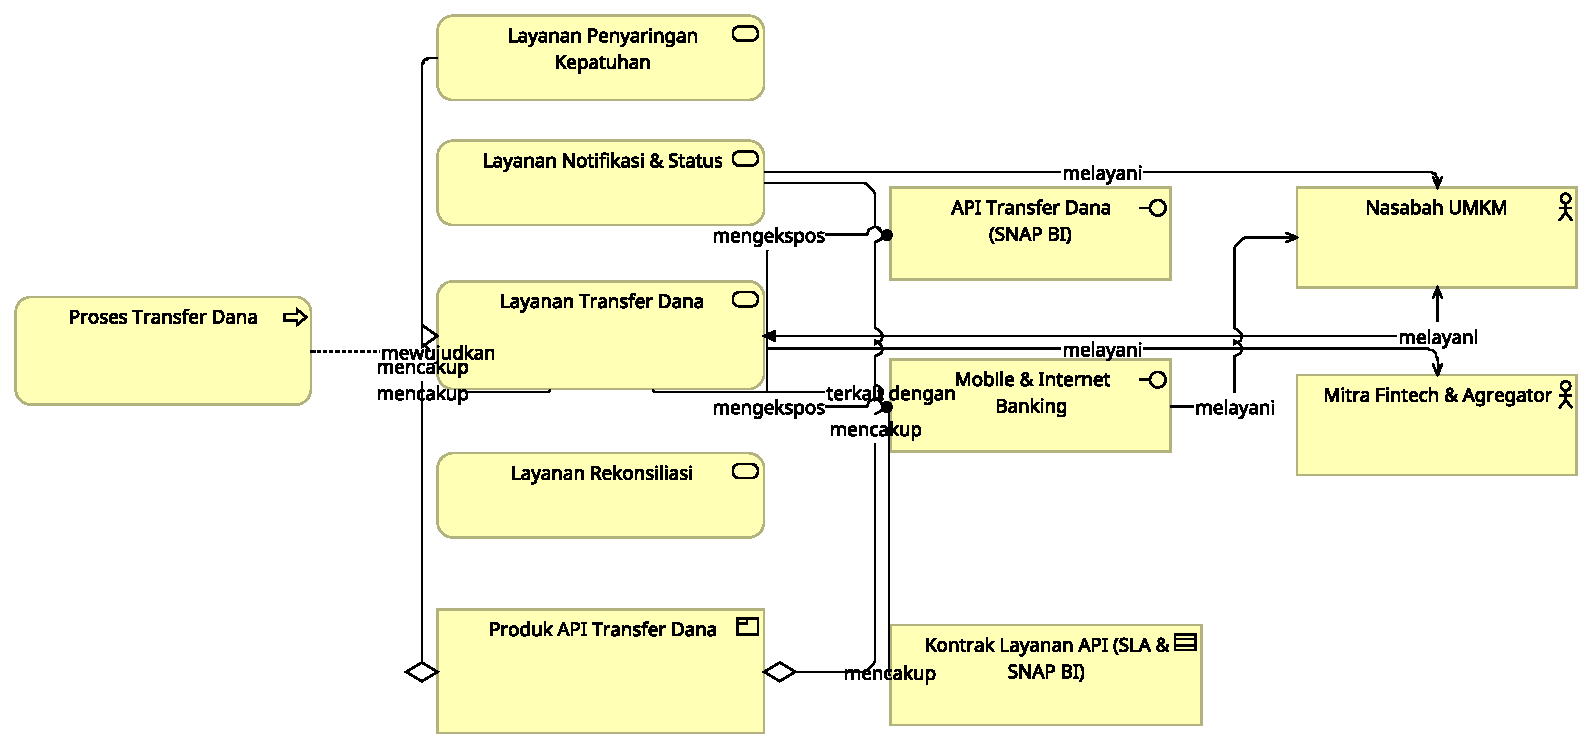
\includegraphics[width=\textwidth,height=.84\textheight,keepaspectratio]{business-overview.pdf}\\
  {\scriptsize Ikhtisar lapisan bisnis: proses $\rightarrow$ layanan $\rightarrow$
  aktor; produk membungkus layanan \& kontrak.}
\end{frame}

\begin{frame}{}
  \centering
  \vspace{1mm}
  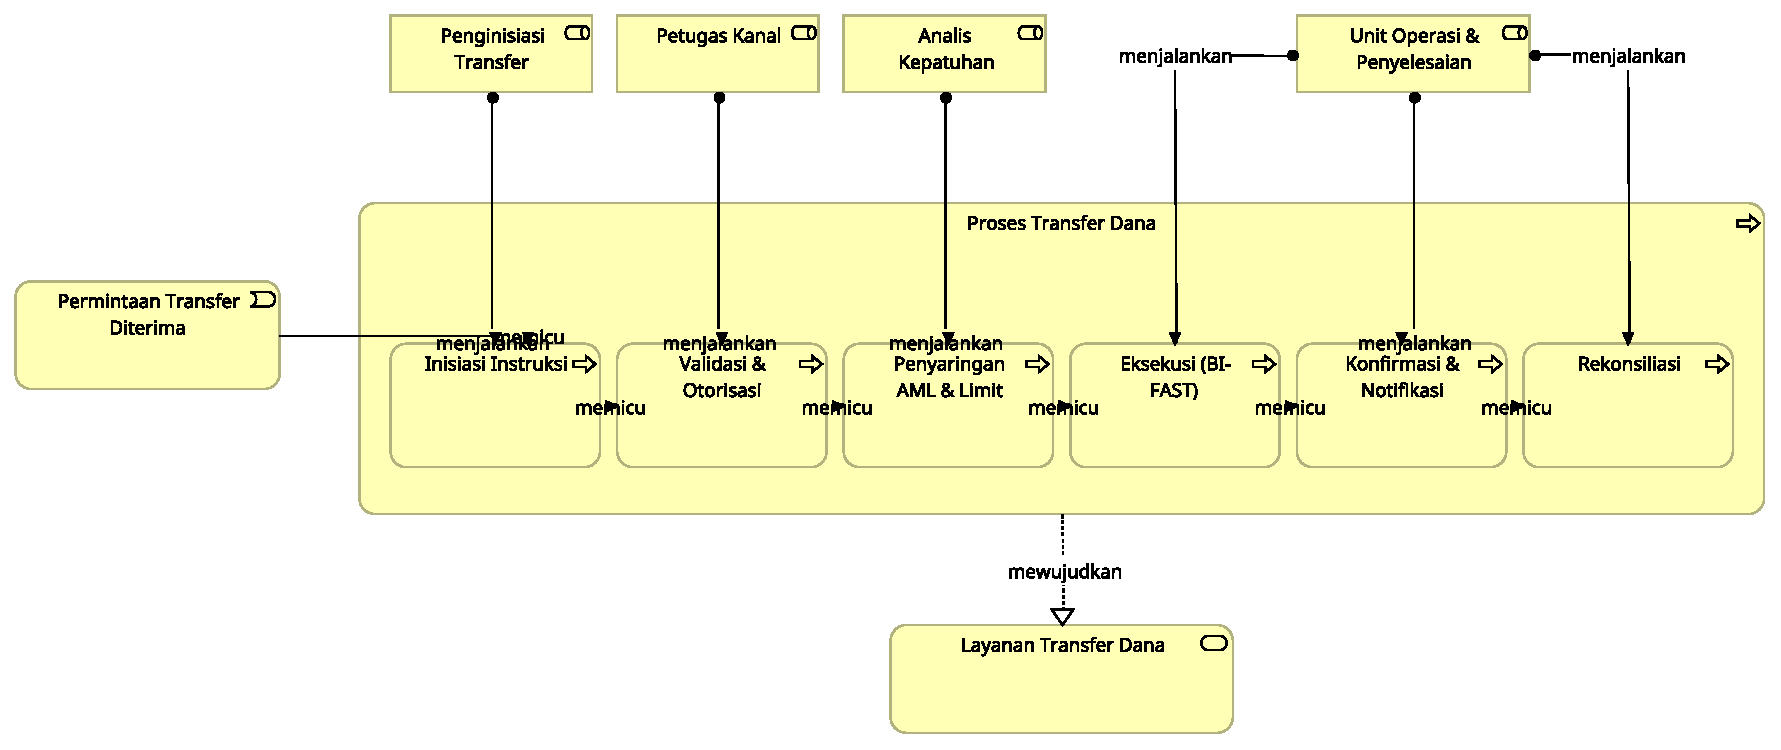
\includegraphics[width=\textwidth,height=.84\textheight,keepaspectratio]{business-transfer.pdf}\\
  {\scriptsize Proses Transfer Dana: peristiwa memicu enam tahap, dijalankan
  peran bisnis, merealisasikan Layanan Transfer Dana.}
\end{frame}

\begin{frame}{Cara Membaca Diagram Bisnis}
  \vspace{4pt}
  \footnotesize
  \begin{itemize}\setlength{\itemsep}{2.5pt}
    \item \textbf{Realisasi:} Proses Transfer Dana \emph{merealisasikan} Layanan
          Transfer Dana.
    \item \textbf{Serving:} layanan \emph{melayani} Nasabah UMKM \& Mitra lewat
          antarmuka API (SNAP BI) dan \emph{mobile banking}.
    \item \textbf{Triggering:} peristiwa ``Permintaan Transfer Diterima'' memicu
          enam tahap berurutan.
    \item \textbf{Assignment:} tiap tahap ditugaskan ke peran (penginisiasi,
          petugas kanal, analis kepatuhan, unit operasi).
    \item \textbf{Access:} tahap menulis/membaca objek bisnis (Instruksi, Hasil
          Penyaringan, Catatan Transaksi/Rekonsiliasi).
  \end{itemize}
  \takeaway{Fungsi bisnis \emph{merealisasikan} kapabilitas strategi, dan proses
  \emph{merealisasikan} value stream---lapisan bisnis menurunkan strategi.}
\end{frame}

% ============================================================
\section{Latihan dan Jembatan}
\sectionframe{Latihan dan Jembatan}

\begin{frame}{Latihan Terapan Individual}
  \vspace{8pt}
  \begin{itemize}
    \item \textbf{Latihan 5.1} -- Capability map studi kasus (inti, pendukung,
          tata kelola).
    \item \textbf{Latihan 5.2} -- Value stream dan proses prioritas beserta
          \emph{pain point}.
    \item \textbf{Latihan 5.3} -- Matriks literatur untuk lapisan bisnis.
    \item \textbf{Latihan 5.4} -- Draft \emph{Literature Review} v1.
  \end{itemize}
  \takeaway{Semua latihan menjadi bahan langsung analisis dan tinjauan pustaka
  makalah.}
\end{frame}

\begin{frame}{Jembatan ke Bab Berikutnya}
  \vspace{8pt}
  \begin{itemize}
    \item Bab berikutnya memperdalam \textbf{lapisan teknis}, dimulai dari
          \textbf{Data Architecture}.
    \item Capability map menunjukkan kapabilitas yang \emph{membutuhkan data};
          value stream menunjukkan titik \emph{aliran} dan \emph{perpindahan}
          data.
    \item Pembahasan data tidak dimulai dari tabel basis data, melainkan dari
          kebutuhan bisnis yang sudah terlihat.
  \end{itemize}
  \takeaway{Lapisan bisnis yang jelas adalah pintu masuk ke arsitektur data,
  aplikasi, dan teknologi.}
\end{frame}

\begin{frame}{\hfill}
  \centering
  \Huge{\textbf{Terima kasih}}\\[8pt]
  \normalsize Pertanyaan \& diskusi
\end{frame}

\end{document}
